\section{Introdução}
%\index{Introdução}%

A integral definida pode ser interpretada como a \'area da regi\~ao limitada pelo gr\'afico de uma fun\c{c}\~ao e o plano de refer\^encia (ou eixo) das vari\'aveis livres. 
Essa \'area tem sinal positivo se estiver acima do plano de refer\^encia, e, sinal negativo se estiver abaixo do plano de refer\^encia.

No caso de uma fun\c{c}\~ao de uma \'unica vari\'{a}vel, a integral definida no intervalo $[a, b]$ \'e representada por 

\begin{equation}
 I = \int_a^b \, f\,(x) \, dx
\end{equation}

\noindent
e indicada como a \'area entre o gr\'afico da fun\c{c}\~ao, $f(x)$, o eixo dos $x$ e as retas $x = a$ e $x = b$ (Figura \ref{fig:intro1}).

\begin{figure}[htb]
 \centering
    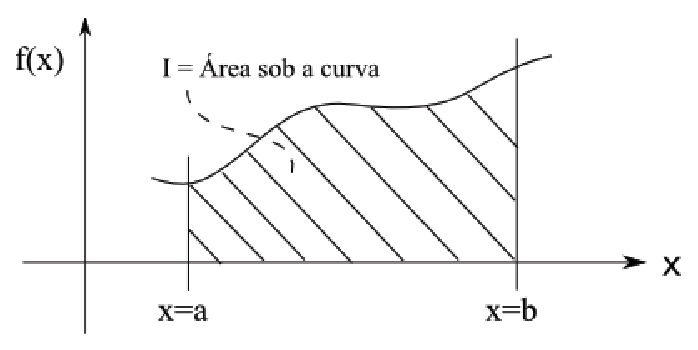
\includegraphics[scale=0.8]{capitulos/capitulo2/figuras/intro1.eps}
    \caption{\'Area sob a curva representando a integral}
    \label{fig:intro1}
\end{figure}

No caso de uma fun\c{c}\~ao de duas vari\'{a}veis, a integral definida em uma regi\~{a}o do plano \'e representada por

\begin{equation}
   I = \displaystyle \int_a^b \, \int_{u\,(x)}^{v\,(x)} \, f\,(x,\,y) \, dy \, dx
\end{equation}

\noindent
e indicada como o volume entre o gr\'afico da fun\c{c}\~ao, $f(x,y)$, o plano $xy$, os planos $x = a$ e $x = b$ e as superf\'icies $y = u(x)$ e $y = v(x)$ (Figura \ref{fig:intro2}).

\begin{figure}[htb]
 \centering
    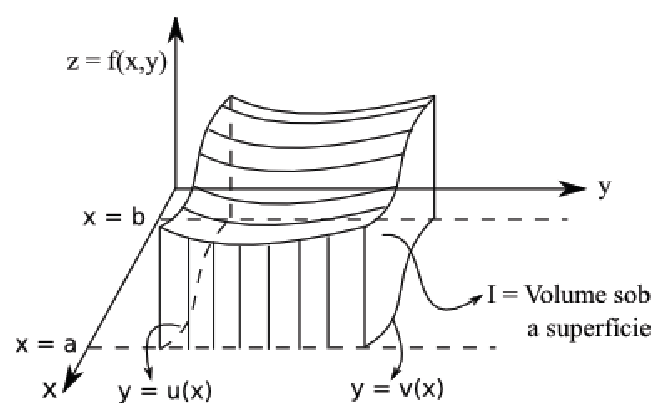
\includegraphics[scale=0.8]{capitulos/capitulo2/figuras/intro2.eps}
    \caption{Volume sob a superfície representando a integral}
    \label{fig:intro2}
\end{figure}

A integra\c{c}\~ao num\'erica pode ser usada tanto para integrar fun\c{c}\~oes anal\'iticas, quanto para integrar fun\c{c}\~oes apresentadas em forma tabular, quando se deseja o valor num\'erico da integral.

\paragraph{Filosofia geral dos m\'etodos de integra\c{c}\~ao}

A filosofia geral dos m\'etodos de integra\c{c}\~ao \'e substituir o integrando por uma fun\c{c}\~ao polinomial que aproxime o gr\'afico da fun\c{c}\~ao a ser integrada. Essa id\'eia est\'a representada na equa\c{c}\~ao \ref{eq:filosofia_geral}

\begin{equation}
   I = \int_a^b \, f\,(x) \, dx \approx \int_a^b \, g\,(x) \, dx
   \label{eq:filosofia_geral}
\end{equation}

\noindent
onde $g(x)$ \'e o polin\^omio de substitui\c{c}\~ao de grau adequadamente escolhido.

